\section{The audit of the saved model versions}
\label{sec:results}

\emph{This section is filled from \texttt{results/paper2/summary/} when the
audit of the saved versions finishes on Colab: the pass counts by check and data
set, every check across versions, the models' stated response to the zone price
deviations against the measured one, and the main test. The figure and
table code is in \texttt{paper2/figs/real.py} and has been run end to end.}

\IfFileExists{generated/tab_real_pass.tex}{%
\begin{table}[t]\centering
\caption{\textbf{Pass counts by check and data set.}}\label{tab:realpass}
\footnotesize\begin{tabular}{@{}lrrrrrrrrr@{}}
\toprule
Data & Versions & Windows & C1 & C2 & C3 & C4 & C5 & C6 & All \\
\midrule
M5 & 31 & 31 & 31/31 & 22/31 & 3/27 & 0/31 & 0/31 & 0/6 & 0/31 \\
Dominick's & 279 & 540 & 68/540 & 423/540 & 209/224 & 16/540 & 345/540 & 5/18 & 0/540 \\
Frat & 184 & 362 & 38/362 & 325/362 & 362/362 & 326/362 & 362/362 & 6/6 & 35/362 \\
\bottomrule
\end{tabular}
\end{table}
\begin{table}[t]\centering
\caption{\textbf{The main test.}}\label{tab:realmain}
\footnotesize\begin{tabular}{@{}lrrrrrrr@{}}
\toprule
 & \multicolumn{5}{c}{Version and window} & \multicolumn{2}{c}{Version} \\
\cmidrule(lr){2-6}\cmidrule(l){7-8}
Score & M5 & Dom. & Frat & Pooled & $p$ & Pooled & $p$ \\
\midrule
Checks passed & $-0.32$ & $-0.19$ & $0.26$ & $-0.08$ & 0.205 & $-0.19$ & 0.004 \\
C1 violation & $0.10$ & $-0.18$ & $-0.41$ & $-0.17$ & 0.007 & $-0.03$ & 0.664 \\
C2 agreement after randomising & $-0.11$ & $0.20$ & $-0.02$ & $0.02$ & 0.740 & $0.01$ & 0.842 \\
C3 seed agreement & $-0.07$ & $0.32$ & $0.30$ & $0.18$ & 0.010 & $-0.01$ & 0.938 \\
C4 share lower & $-0.06$ & $-0.04$ & $-0.18$ & $-0.09$ & 0.159 & $-0.01$ & 0.916 \\
C5 rank & $-0.19$ & $-0.32$ & $-0.75$ & $-0.42$ & 0.000 & $-0.32$ & 0.000 \\
C5 bias & $0.62$ & $0.03$ & $0.70$ & $0.45$ & 0.000 & $0.36$ & 0.000 \\
C6 agreement with LightGBM & $-0.31$ & $-0.48$ & $0.20$ & $-0.20$ & 0.394 & $-0.20$ & 0.392 \\
Checks passed, C5 left out$^\dagger$ & $-0.32$ & $-0.04$ & $0.26$ & $-0.03$ & 0.615 & $-0.13$ & 0.055 \\
Checks passed, C1 and C5 left out$^\dagger$ & $-0.32$ & $-0.10$ & $0.15$ & $-0.09$ & 0.163 & $-0.15$ & 0.032 \\
\bottomrule
\end{tabular}
\end{table}
\begin{figure*}[t]\centering
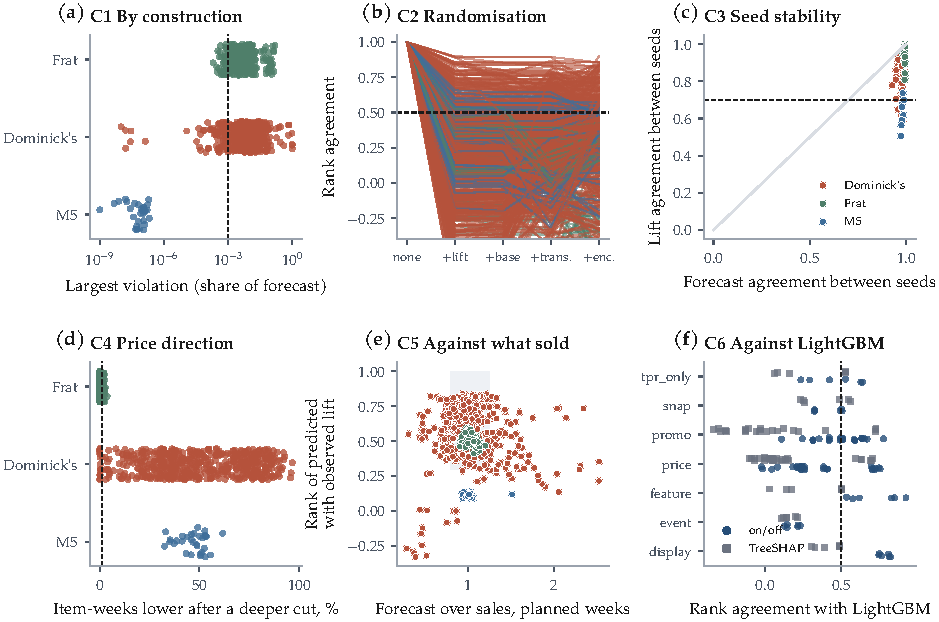
\includegraphics[width=\textwidth]{figs/fig_real_checks.pdf}
\caption{\textbf{Every check across every audited version.}}\label{fig:realchecks}
\end{figure*}
\begin{figure*}[t]\centering
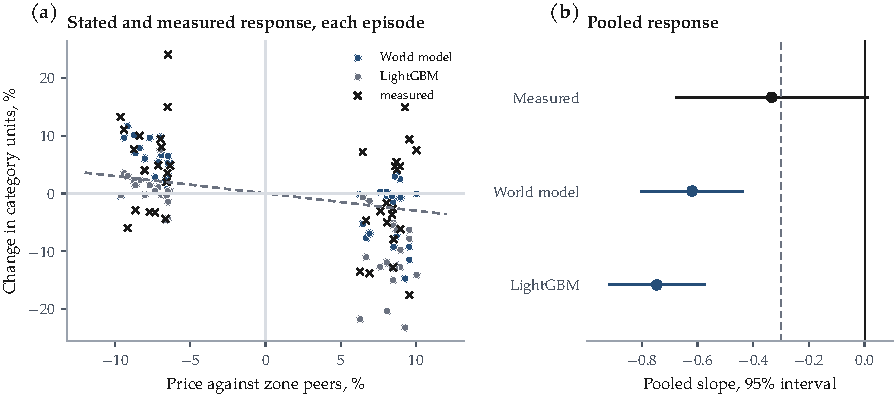
\includegraphics[width=\textwidth]{figs/fig_real_c7.pdf}
\caption{\textbf{Stated against measured response to zone price deviations.}}\label{fig:realc7}
\end{figure*}
\begin{figure*}[t]\centering
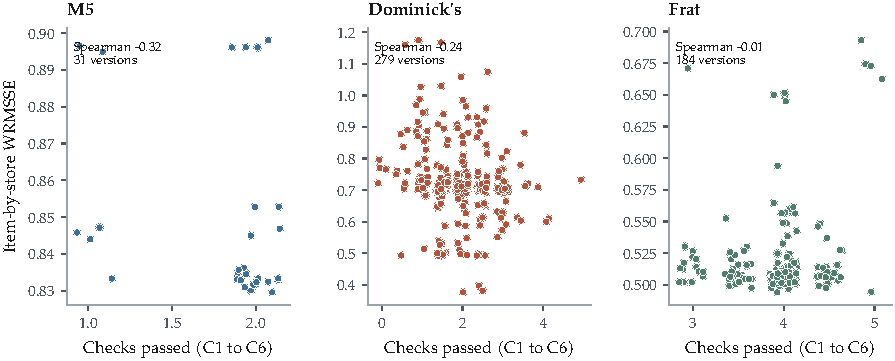
\includegraphics[width=\textwidth]{figs/fig_real_main.pdf}
\caption{\textbf{Checks passed against accuracy.}}\label{fig:realmain}
\end{figure*}
}{}
